\documentclass[12pt]{article}
\usepackage[english]{babel}
\usepackage[letterpaper,top=2cm,bottom=2cm,left=3cm,right=3cm,marginparwidth=1.75cm]{geometry}
\usepackage{amsmath}
\usepackage{amsfonts}
\usepackage{graphicx}
\usepackage{float}
\DeclareMathOperator{\pv}{pv}
\DeclareMathOperator{\pva}{pva}
\renewcommand{\theenumi}{\alph{enumi}}
\makeatletter
\renewcommand{\thesection}{Question \arabic{section}}
\renewcommand{\thesubsection}{\arabic{subsection}}
\makeatother
\title{FINC-UB 1 Homework 5}
\author{Ishan Pranav}
\date{October 6, 2023}
\begin{document}
\maketitle
\section{}
Let $\mu$ represent the expected return of a security and $\sigma$ be its standard deviation.
\begin{enumerate}
    \item
    \begin{enumerate}
        \item[i.] Note $\mu_Z=15\%$, and $\sigma_Z=20\%$.
        \item[ii.]
        \begin{align*}
        \mu
        &=0.75\mu_Z+0.25\mu_Y\\
        &=(0.75\times 15\%)+(0.25\times 35\%)\\
        &=20\%.
        \end{align*}
        \begin{align*}
        \sigma
        &=\sqrt{(0.75)^2\sigma_Z^2+(0.25)^2\sigma_Y^2+2\rho_{Z,Y}(0.75)(0.25)\sigma_Z\sigma_Y}\\
        &=\sqrt{(0.75)^2(20\%)^2+(0.25)^2(40\%)^2+2(0.25)(0.75)(0.25)(20\%)(40\%)}\\
        &=20\%.
        \end{align*}
        \item[iii.]
        \begin{align*}
        \mu
        &=0.5\mu_Z+0.5\mu_Y\\
        &=(0.5\times 15\%)+(0.5\times 35\%)\\
        &=25\%.
        \end{align*}
        \begin{align*}
        \sigma
        &=\sqrt{(0.5)^2\sigma_Z^2+(0.5)^2\sigma_Y^2+2\rho_{Z,Y}(0.5)(0.5)\sigma_Z\sigma_Y}\\
        &=\sqrt{(0.5)^2(20\%)^2+(0.5)^2(40\%)^2+2(0.25)(0.5)(0.5)(20\%)(40\%)}\\
        &\approx 24.4949\dots\%.
        \end{align*}
        \item[iv.]
        \begin{align*}
        \mu
        &=0.25\mu_Z+0.75\mu_Y\\
        &=(0.25\times 15\%)+(0.75\times 35\%)\\
        &=30\%.
        \end{align*}
        \begin{align*}
        \sigma
        &=\sqrt{(0.25)^2\sigma_Z^2+(0.75)^2\sigma_Y^2+2\rho_{Z,Y}(0.25)(0.75)\sigma_Z\sigma_Y}\\
        &=\sqrt{(0.25)^2(20\%)^2+(0.75)^2(40\%)^2+2(0.75)(0.25)(0.25)(20\%)(40\%)}\\
        &\approx 31.6228\dots\%.
        \end{align*}
        \item[v.] Note $\mu_Y=35\%$, and $\sigma_Y=40\%$.
    \end{enumerate}
    \item See Figure 1.
    \begin{figure}[h]
    \begin{center}
    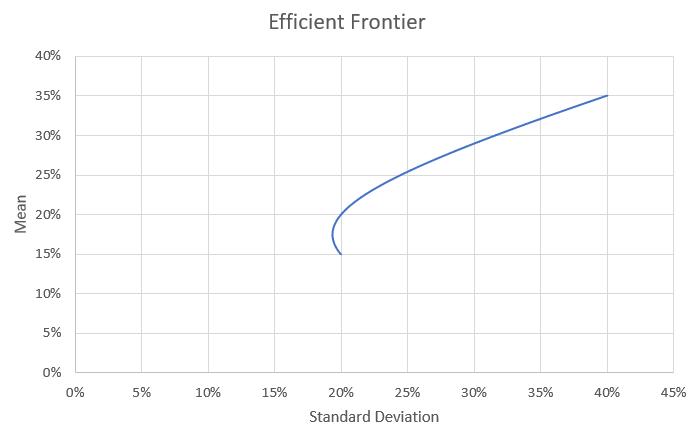
\includegraphics[width=4in]{images/efficient-frontier.png}
    \end{center}
    \caption{The mean--standard deviation frontier for Securities Z and Y.\label{fig:ios}}
    \end{figure}
    \item Based on Figure 1, a rational investor would prefer a portfolio with around 61\% invested in Security Z and around 39\% invested in Security X. This ideal portfolio's Sharpe ratio is about 1.0328. Of the options above, portfolio (iii) is the best; it's Sharpe ratio is about 1.0206.
\end{enumerate}
\section{}
Let $\mu$ represent the expected return of a security and $\sigma$ be its standard deviation.
\begin{enumerate}
    \item The expected return of a portfolio invested only in the risk-free asset is $8\%$, and its standard deviation is 0. 
    \item\begin{align*}
    \mu
    &=0.5\mu_F+0.5\mu_M\\
    &=(0.5\times 8\%)+(0.5\times 16\%)\\
    &=12\%.
    \end{align*}
    Note that the market is entirely uncorrelated with the risk-free asset, so $\rho_{F,M}=0$, and that the risk-free asset has no variance.
    \begin{align*}
    \sigma
    &=\sqrt{(0.5)^2\sigma_F^2+(0.5)^2\sigma_M^2+2\rho_{F,M}(0.5)(0.5)\sigma_F\sigma_M}\\
    &=\sqrt{0+(0.5)^2\sigma_M^2+0}\\
    &=0.5\times 10\%\\
    &=5\%.
    \end{align*}
    The expected return is 12\%, and the standard deviation is 5\%.
    \item\begin{align*}
    \mu
    &=-0.25\mu_F+1.25\mu_M\\
    &=(-0.25\times 8\%)+(1.25\times 16\%)\\
    &=18\%.
    \end{align*}
    \begin{align*}
    \sigma
    &=\sqrt{(-0.25)^2\sigma_F^2+(1.25)^2\sigma_M^2+2\rho_{F,M}(-0.25)(1.25)\sigma_F\sigma_M}\\
    &=\sqrt{0+(1.25)^2\sigma_M^2+0}\\
    &=1.25\times 10\%\\
    &=12.5\%.
    \end{align*}
    The expected return is 18\%, and the standard deviation is 12.5\%.
    \item 
    \begin{align*}
    2\times 10\%
    &=\sqrt{(1-w_M)^2\sigma_F^2+w_M^2\sigma_M^2+2\rho_{F,M}w_M(1-w_M)\sigma_F\sigma_M}\\
    &=\sqrt{0+w_M^2\sigma_M^2+0}\\
    &=w_M\times 10\%.
    \end{align*}
    A portfolio must invest 200\% of its wealth in the S\&P 500, financed by borrowing 100\% of its wealth at the risk-free rate to achieve a standard deviation that is double that of the S\&P 500. 

    The expected return on that portfolio is $(200\%\times 16\%)+(-100\%\times 8\%)=24\%$.
\end{enumerate}
\section{}
We can compare portfolios using their Sharpe ratio. The portfolio with the highest Sharpe ratio will combine most effectively with the risk-free Treasury bill to produce an optimal allocation.

\begin{enumerate}
    \item The Sharpe ratio of the Russell Fund is $\frac{16\%-6\%}{12\%}=0.8\bar{3}.$
    \item The Sharpe ratio of the Windsor Fund is $\frac{14\%-6\%}{10\%}=0.8.$
    \item The Sharpe ratio of the S\&P Fund is $\frac{12\%-6\%}{8\%}=0.75.$
    \item The expected value of the portfolio is ($60\%\times 16\%)+(40\%\times 12\%)=14.4\%$, and its standard deviation is $\sqrt{(60\%)^2(12\%)^2+(40\%)^2(8\%)^2+2(0.7)(60\%)(40\%)(12\%)(8\%)}\approx 9.713\dots\%$. Thus the Sharpe ratio of the portfolio is $\frac{14.4\%-6\%}{.0971\dots\%}\approx 0.8648\dots$
\end{enumerate}
As rational investors, we appreciate returns and are averse to volatility. The optimal portfolio is the one that offers the greatest excess return for each additional unit of volatility---that is, the one with the greatest Sharpe ratio. Based on the above choices, we prefer portfolio (d) which combines the Russell Fund and the S\&P Fund.
\section{}
\begin{enumerate}
    \item As the expected return of Asset 3 increases, the share of Asset 3 in the minimum variance efficient (MVE) portfolio increases. This is because Asset 3 provides more utility to investors, who maximize expected returns. As Asset 3's expected returns per unit of risk increase relative to those of its alternatives, increasing the share of Asset 3 in the MVE portfolio improves it. 
    \item As the standard deviation of the returns of Asset 3 increases, the share of Asset 3 in the MVE portfolio decreases. This is because Asset 3 provides less utility to investors, who minimize volatility. As Asset 3's expected returns per unit of risk decrease relative to those of its alternatives, decreasing the share of Asset 3 in the MVE portfolio improves it.
    \item As the standard deviation of the returns of Asset 2 increases, the share of Asset 3 in the MVE portfolio increases. This is because Asset 2 now provides less utility to investors relative to its alternatives. Asset 3 is an alternative to Asset 2. Thus, increasing the share of Asset 3 in the MVE portfolio improves it.
    \item As the correlation between Assets 2 and 5 increases, the share of Asset 3 in the MVE portfolio first increases then decreases.
\end{enumerate}
\section{}
Each asset in the market portfolio is weighted based on its market value (market capitalization). The market capitalization of Asset A is $n_Ap_A=25\times\$2=\$50$ and the market capitalization of Asset B is $n_Bp_B=50\times\$5=\$250$. Since Assets A and B are the only assets in the market, the total market capitalization of the entire market is $\$50+\$250=\$300$. Thus the weight of Asset A is $w_A=\frac{n_Ap_A}{n_Ap_A+n_Bp_B}=\frac{\$50}{\$300}=16.\bar{6}\%$ and the weight of Asset B is $w_B=\frac{n_Bp_B}{n_Ap_A+n_Bp_B}=\frac{\$250}{\$300}=83.\bar{3}\%$.
\section{}
\begin{enumerate}
    \item The excess return on the market portfolio is $12\%-4\%=8\%$. 
    \item If a certain stock has a realized return of 14\%, we cannot make any claim about its $\beta$. The coefficient $\beta$ can be expressed as the ratio of the expected excess return of the stock to the expected excess return of the market. An individual realized return of 14\% does not give any information about the expected return. 
    \item If a certain stock has an expected return of 14\%, then its excess return is $14\%-4\%=10\%$, and it thus has $\beta=\frac{10\%}{8\%}=1.25$.
\end{enumerate}
\section{}
\begin{enumerate}
    \item Equation (1) is used to determine the expected return on an individual security. That expected return is $0.06+(0.15-0.06)\times 2=0.22$, or 22\%.
    \item Equation (2) is used to determine the expected return on a portfolio knowing that it is an efficient portfolio consisting of the market portfolio combined with a risk-free security. The expected return of a portfolio with the same volatility as the market is the expected return of the market, 0.15, or 15\%.
    \item The portfolio in part (b) \textit{is} the market portfolio, so it has $\beta=1$.
    \item Equation (1) can be used to determine the expected excess return of an individual security in the market portfolio. Equation (2) can be used to determine the expected excess return of an efficient portfolio that combines the market portfolio with a risk-free security.
\end{enumerate}
\section{}
\begin{enumerate}
    \item Intuitively, a stock with $\beta=0$ has no covariance with the market. Such a stock is free of systematic risk and is thus indistinguishable from a risk-free security. This implies that its expected return is equal to the risk-free rate under the capital asset pricing model.
    \item Theoretically, a stock with $\beta<0$ is possible but highly unlikely since this requires the stock to have an inverse relationship with the market portfolio (which contains the stock). An inverse broad-market index fund that ``bets against'' the market portfolio could have $\beta<0$ by construction. Other assets with $\beta<0$ might include gold, which experiences above-average returns when the market experiences below-average returns; still, all assets tend to increase in value over time in conjunction with inflation.
\end{enumerate}
\end{document}